\SourcePage{701}{706}
\section{Multipole moments of hadrons}

We now consider the transition current represented by a diagram of the same form as~(138.2):
\begin{equation}
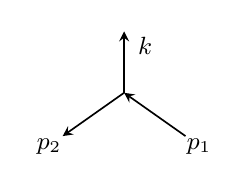
\begin{tikzpicture}[baseline=-.45ex,x=1cm,y=1cm,>=stealth,line width=.6pt,font=\small]
  \coordinate (v) at (0,0);
  \draw[->] (.78,-.55)--(v);
  \draw[->] (v)--(-.78,-.55);
  \draw[->] (v)--(0,.78);
  \node[below right] at (.67,-.46) {$p_1$};
  \node[below left] at (-.67,-.46) {$p_2$};
  \node[right] at (.05,.60) {$k$};
\end{tikzpicture}
\tag{142.1}
\end{equation}
Here, however, the lines $p_1$ and~$p_2$ correspond to different particles (with masses $M_1$ and~$M_2$); it is more convenient to draw the photon line $k=p_1-p_2$ as leaving the vertex. The photon may now be either virtual or real: the only restriction is $k^2<(M_1-M_2)^2$, so $k^2=0$ is allowed. The processes described by this diagram therefore include, in particular, photon emission accompanying transformations of particles, including nuclei (in the latter case the initial and final particles are the nucleus in different states).

Of greatest interest for the question at hand is the case in which the photon wavelength is large in comparison with the characteristic ``dimensions'' of the particle (that is, the dimensions entering its form factors; for a nucleus they of course coincide with its ``radius''). The transition current can then be expanded in powers of~$k$\footnote{We follow below the method proposed by \emph{V.~B. Berestetskii} (1948).}.

First, we note that
\begin{equation}
J_{fi}=0\qquad\text{when}\qquad k=0.
\tag{142.2}
\end{equation}

\SourcePage{702}{707}
Indeed, the limit $k\to0$ corresponds to a potential constant in space and time. Such a potential, however, has no physical significance and cannot cause any real process. The same conclusion can also be reached more formally. The currents considered in~\S~138 were nonzero at $k=0$ because of terms proportional to the 4-vector $P=p_1+p_2$; when $M_1\ne M_2$, however, $(Pk)\ne0$, and the transversality condition on the current therefore forbids such terms.

In three-dimensional form, the transversality condition for the current $J_{fi}=(\rho_{fi},\mathbf J_{fi})$ is
\begin{equation}
\mathbf k\mathbf J_{fi}=\omega\rho_{fi}.
\tag{142.3}
\end{equation}
It may be satisfied in either of two ways:
\begin{equation}
\mathbf J_{fi}=\omega\mathbf v(\mathbf k,\omega),\qquad
\rho_{fi}=\mathbf k\mathbf v(\mathbf k,\omega),
\tag{142.4}
\end{equation}
or
\begin{equation}
\mathbf J_{fi}=\mathbf k\times\mathbf a(\mathbf k,\omega),\qquad
\rho_{fi}=0.
\tag{142.5}
\end{equation}
Here $\mathbf v$ is some polar vector, while $\mathbf a$ is an axial vector. The current is said to be of electric type in the first case and of magnetic type in the second. According to~(142.2), $\mathbf v$ and~$\mathbf a$ remain finite or tend to zero as $\mathbf k,\omega\to0$.

Let the photon energy satisfy $\omega\ll M_1$. The recoil may then be neglected, and the final particle~$M_2$ may also be regarded as being at rest (in the rest frame of the particle~$M_1$); $\omega$ is then fixed: $\omega=M_1-M_2$. The states of the stationary particles $M_1$ and~$M_2$ are characterized by three-dimensional spinors $w_1$ and~$w_2$ of ranks $2s_1$ and~$2s_2$, where $s_1$ and~$s_2$ are the particle spins. The transition current must be a bilinear combination of $w_1$ and~$w_2^*$. From products of the components of these spinors one can construct irreducible tensors of ranks $l=s_1+s_2,\ldots,|s_1-s_2|$ (for a specified~$l$ this will be a true tensor or a pseudotensor, according to the intrinsic parities of the particles $M_1$ and~$M_2$). Apart from these tensors, the only quantity at our disposal is the vector~$\mathbf k$. To construct the first term in the expansion of the current in powers of~$\mathbf k$, these quantities must be used to form a vector of the lowest possible degree in~$\mathbf k$. This is achieved by taking the tensor of lowest rank and contracting it scalarly $l-1$ times with the vector~$\mathbf k$. The result is the polar vector~$\mathbf v$ or the axial vector~$\mathbf a$.

Let $Q_{lm}$ be the spherical components of the tensor formed from the particle wave amplitudes. The spherical components of the rank-$(l-1)$ tensor made from the components of~$\mathbf k$ are $|\mathbf k|^{l-1}Y_{l-1,m}(\mathbf n)$, where $\mathbf n=\mathbf k/\omega$. By the general rule for coupling spherical tensors (see~III, (107.3)), the spherical components

\SourcePage{703}{708}
of the vector $\mathbf v$ may be written as
\[
\begin{aligned}
v_\lambda={}&(-1)^{\lambda+1}i^l\frac{\sqrt{4\pi}}{(2l-1)!!}
\sqrt{\frac{2l+1}{l}}\,|\mathbf k|^{l-1}\times{}\\
&\times\sum_m
\begin{pmatrix}
l-1&1&l\\
\lambda+m&-\lambda&-m
\end{pmatrix}
Q_{l,-m}Y_{l-1,\lambda+m}(\mathbf n),
\end{aligned}
\]
where $\lambda$ takes the values $0,\ \pm1$ (the choice of the overall factor is discussed below). Using formulas~(7.16), we can express $\mathbf v$ in terms of vector spherical harmonics:
\begin{equation}
\begin{aligned}
\mathbf v={}&i^l\frac{\sqrt{4\pi}\,|\mathbf k|^{l-1}}
{(2l-1)!!\sqrt{l(2l+1)}}\sum_m(-1)^{l-m}Q_{l,-m}\times{}\\
&\times\left[\sqrt{l+1}\,\mathbf Y_{lm}^{(\mathrm e)}(\mathbf n)
+\sqrt l\,\mathbf Y_{lm}^{(\mathrm l)}(\mathbf n)\right].
\end{aligned}
\tag{142.6}
\end{equation}
Substitution in~(142.4) gives the $El$ transition current:
\begin{equation}
\begin{aligned}
\mathbf J_{fi}={}&i^l\frac{\sqrt{4\pi}\,|\omega|\,|\mathbf k|^{l-1}}
{(2l-1)!!\sqrt{l(2l+1)}}\sum_m(-1)^{l-m}Q_{l,-m}^{(\mathrm e)}\times{}\\
&\times\left[\sqrt{l+1}\,\mathbf Y_{lm}^{(\mathrm e)}(\mathbf n)
+\sqrt l\,\mathbf Y_{lm}^{(\mathrm l)}(\mathbf n)\right],
\end{aligned}
\tag{142.7}
\end{equation}
\begin{equation}
\rho_{fi}=i^l\frac{\sqrt{4\pi}\,|\mathbf k|^l}
{(2l-1)!!\sqrt{l(2l+1)}}
\sum_m(-1)^{l-m}Q_{l,-m}^{(\mathrm e)}Y_{lm}(\mathbf n)
\tag{142.8}
\end{equation}
(we distinguish $|\mathbf k|$ from~$\omega$ throughout, since the formulas may be applied to both real and virtual photons, for which these quantities do not coincide).

In~(142.7), (142.8), the spherical tensor $Q_{lm}$ (denoted there by $Q_{lm}^{(\mathrm e)}$) is understood to be a true tensor. If it is instead a pseudotensor (which we then denote by $Q_{lm}^{(\mathrm m)}$), formula~(142.6) determines the pseudovector~$\mathbf a$. Substitution in~(142.5) then gives the $Ml$ transition current:
\begin{equation}
\begin{aligned}
\mathbf J_{fi}&=i^l\frac{\sqrt{4\pi}}{(2l-1)!!}
\sqrt{\frac{l+1}{l(2l+1)}}\,|\mathbf k|^l
\sum_m(-1)^{l-m}Q_{l,-m}^{(\mathrm m)}\mathbf Y_{lm}^{(\mathrm m)}(\mathbf n),\\
\rho_{fi}&=0.
\end{aligned}
\tag{142.9}
\end{equation}
The quantities $Q_{lm}^{(\mathrm e)}$ and~$Q_{lm}^{(\mathrm m)}$ are the electric and magnetic multipole transition moments of the hadron. Their role in hadron electrodynamics is entirely analogous to that played by the corresponding quantities in electron electrodynamics. However, whereas

\SourcePage{704}{709}
for electronic systems these moments can, in principle, be calculated from wave functions (as matrix elements of the appropriate operators), in hadron electrodynamics they are phenomenological quantities whose values must be obtained experimentally.

The normalization adopted for these quantities in~(142.7)--(142.9) agrees with their definition in~\S~46. This can be verified by treating the currents~(142.7)--(142.9) as Fourier components of the transition current in coordinate representation. For example, expand the factor $e^{-i\mathbf k\mathbf r}$ in the integral
\begin{equation}
\rho_{fi}(\mathbf k)=\int\rho_{fi}(\mathbf r)e^{-i\mathbf k\mathbf r}\,d^3x
\tag{142.10}
\end{equation}
with formula~(46.3). This gives
\[
\rho_{fi}(\mathbf k)=4\pi i^l\sum_{l,m}Y_{lm}(\mathbf n)
\int\rho_{fi}(\mathbf r)Y^*_{lm}\left(\frac{\mathbf r}{r}\right)
g_l(|\mathbf k|r)\,d^3x.
\]
Retaining the term with the smallest~$l$ for which the integral is nonzero, and replacing $g_l(|\mathbf k|r)$ for $|\mathbf k|r\ll1$ by the first term of its expansion~(46.5), we recover formula~(142.9), with
\begin{equation}
Q_{lm}^{(\mathrm e)}=\sqrt{\frac{4\pi}{2l+1}}
\int r^l\rho_{fi}(\mathbf r)Y_{lm}\left(\frac{\mathbf r}{r}\right)d^3x
\tag{142.11}
\end{equation}
in agreement with definition~(46.7).

We shall also show that, when applied to emission of a real photon, the formulas obtained above lead back to results already known to us.

The amplitude for a transition accompanied by emission of a photon of momentum $\mathbf k=\omega\mathbf n$ and polarization $e=(0,\mathbf e)$ is
\begin{equation}
M_{fi}=-e\sqrt{4\pi}\,\mathbf e^*\mathbf J_{fi}.
\tag{142.12}
\end{equation}
If the nucleus has definite values of the angular-momentum projection in the initial and final states ($M_i$ and~$M_f$), only one term remains in the sum over~$m$ in~(142.7)--(142.9): $m=M_i-M_f$. Since, by~(16.23), the products $\mathbf Y_{lm}^{(\mathrm e)}\mathbf e^{(\lambda)*}$ or $\mathbf Y_{lm}^{(\mathrm m)}\mathbf e^{(\lambda)*}$ ($\lambda=\pm1$ is the photon helicity and $\mathbf e^{(\lambda)}\perp\mathbf n$) are proportional to $D_{\lambda m}^l$, we return to the formulas considered in~\S~48.

\SourcePage{705}{710}
The differential radiation probability\footnote{The factor $2\pi\delta$ in this formula, instead of $(2\pi)^4\delta^{(4)}$ in~(64.11), arises because neglecting nuclear recoil removes momentum conservation, leaving only conservation of energy.} is
\begin{equation}
dw=2\pi\delta[\omega-(E_i-E_f)]|M_{fi}|^2\frac{d^3k}{2\omega(2\pi)^3}
\tag{142.13}
\end{equation}
($E_i$, $E_f$ are the initial and final energies of the nucleus). The total probability is obtained by summing over polarizations and integrating over~$d^3k$. Substituting~(142.7) or~(142.9) in~(142.12), and then in~(142.13), and carrying out these operations, we recover formula~(46.9) (or~(47.2)).

Formulas~(142.7)--(142.9) include all cases that can arise in emission of a real photon. For virtual photons, however, one further case is possible which is not described by these formulas (\emph{R.~H. Fowler}, 1930).

If the initial and final states of the nucleus have the same spin and parity, their wave amplitudes can be used to form a scalar~$Q_0$, and hence a transition current of the form
\begin{equation}
\rho_{fi}=Q_0\mathbf k^2,\qquad \mathbf J_{fi}=Q_0\omega\mathbf k.
\tag{142.14}
\end{equation}
The quantity $Q_0$ is called the \emph{monopole} ($E0$) transition moment. The corresponding transition amplitude vanishes for emission of a real photon (because $\mathbf e^*\mathbf k=0$). A monopole current can, however, produce transitions involving emission of a virtual photon. Moreover, it is the only such source when $s_1=s_2=0$, for then all the multipole moments vanish.

The dependence of the monopole current~(142.14) on~$\omega$ and~$\mathbf k$ is analogous to that of the electric quadrupole current. Accordingly, the moment~$Q_0$ is of the same order as the quadrupole moment. The same conclusion follows by interpreting~(142.14) as Fourier components of the current in coordinate representation. Expanding the factor $e^{-i\mathbf k\mathbf r}$ in~(142.10) in powers of~$\mathbf k\mathbf r$ and taking $\rho_{fi}(r)$ to be spherically symmetric, we obtain
\[
\rho_{fi}(\mathbf k)=-\frac16\mathbf k^2\int\rho_{fi}(r)r^2\,d^3x.
\]
Comparison with~(142.14) gives
\begin{equation}
Q_0=-\frac16\int\rho_{fi}(r)r^2\,d^3x.
\tag{142.15}
\end{equation}
The similarity between this quantity and the quadrupole moment is evident.

\SourcePage{706}{711}
\ProblemHeading

\begin{enumerate}
\item Find the probability that an atom is ionized from its $K$~shell by the nuclear excitation energy~$\omega$ (the so-called internal conversion of $\gamma$~radiation) in a nuclear $Ml$ transition, neglecting both the electron binding energy in the atom and the effect of the nuclear field on its wave functions\footnote{This approximation requires a small nuclear charge and sufficiently large excitation energies~$\omega$ (while $1/\omega$ is still assumed large compared with the dimensions of the nucleus). In fact, the approximation is not very satisfactory, and a more accurate calculation requires the nuclear Coulomb field to be taken into account.}.

\SolutionHeading The process is described by the diagram
\begin{equation}
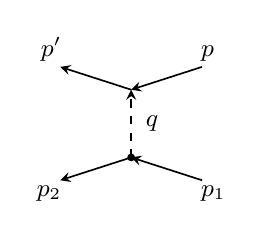
\begin{tikzpicture}[baseline=-.45ex,x=1cm,y=1cm,>=stealth,line width=.6pt,font=\small]
  \coordinate (ve) at (0,.43);
  \coordinate (vn) at (0,-.43);
  \draw[->] (.90,.72)--(ve);
  \draw[->] (ve)--(-.90,.72);
  \draw[dashed,->] (vn)--(ve);
  \draw[->] (.90,-.72)--(vn);
  \draw[->] (vn)--(-.90,-.72);
  \fill (vn) circle (1.4pt);
  \node[above right] at (.76,.66) {$p$};
  \node[above left] at (-.76,.66) {$p'$};
  \node[below right] at (.76,-.66) {$p_1$};
  \node[below left] at (-.76,-.66) {$p_2$};
  \node[right] at (.06,0) {$q$};
\end{tikzpicture}
\tag*{(1)}
\end{equation}
where $p_1$ and~$p_2$ refer to the stationary nucleus in different states, while $p=(m,0)$ and~$p'=(m+\omega,\mathbf p')$ are the 4-momenta of the initial and final electrons. The amplitude corresponding to this diagram is
\[
M_{fi}=-e^2\frac{4\pi}{q^2}\bar u(p')(\gamma J_{fi})u(p),
\]
where $J_{fi}$ is the nuclear transition current. Summing over the final electron polarizations and averaging over the initial ones gives
\[
\frac12\sum_{\text{pol}}|M_{fi}|^2
=e^4\frac{16\pi^2}{(q^2)^2}
\left\{q^2(J_{fi}J_{fi}^*)+4(J_{fi}p)(J_{fi}^*p)\right\}
\]
(we used $J_{fi}q=0$, and hence $J_{fi}p=J_{fi}p'$). The conversion probability is calculated as
\[
dw_{\text{conv}}=2|\psi_i(0)|^2
\left(\frac{|\mathbf p|}{m}\,d\sigma\right)_{\mathbf p\to0},
\]
where $d\sigma$ is the cross section for the scattering represented by diagram~(1), with $p=(\varepsilon,\mathbf p)$, and $\psi_i$ is the wave function of the atomic electron; for a $K$~electron,
\[
|\psi_i(0)|^2=(Z\alpha m)^3/\pi.
\]
The factor~2 accounts for the two electrons in the atom's $K$~shell. The cross section $d\sigma$ is calculated from
\[
d\sigma=2\pi\delta(\varepsilon+\omega-\varepsilon')|M_{fi}|^2
\frac{d^3p'}{2|\mathbf p|\,2\varepsilon'(2\pi)^3}
\]
(cf. the note on p.~710).

For an $Ml$ transition, $J_{fi}$ must be taken from~(142.9). Integration of $dw_{\text{conv}}$ over~$d\varepsilon'$ removes the $\delta$~function, while integration over~$do'$ turns $|\mathbf Y_{lm}^{(\mathrm m)}|^2$ into~1. The conversion probability is consequently expressed through $|Q_{l,-m}^{(\mathrm m)}|^2$. According to~(46.9), however, the probability $w_\gamma$ of spontaneous photon emission in the same nuclear transition is expressed through this same quantity. The final result is
\[
\frac{w_{\text{conv}}}{w_\gamma}
=2\alpha(Z\alpha)^3\frac{m}{\omega}
\left(1+\frac{2m}{\omega}\right)^{l+1/2}
\]
(this ratio is called the \emph{conversion coefficient}).

\SourcePage{707}{712}
\item The same for a nuclear $El$ transition.

\SolutionHeading The same procedure, using the transition current from~(142.7), (142.8), gives
\[
\frac{w_{\text{conv}}}{w_\gamma}
=2\alpha(Z\alpha)^3
\left(1+\frac{4l}{l+1}\frac{m^2}{\omega^2}\right)^{l-1/2}
\frac{m}{\omega}.
\]

\item The same for a monopole transition of the nucleus.

\SolutionHeading Using the transition current from~(142.14), we obtain
\[
w_{\text{conv}}=4\alpha^2(Z\alpha)^3m^3\omega^2
\left(1+\frac{2m}{\omega}\right)^{3/2}|Q_0|^2.
\]
Since monopole photon emission is impossible, $|Q_0|^2$ cannot be eliminated from this expression.
\end{enumerate}
